\subsubsection{T5}

In Transfer Learning, we start by training our model in an unsupervised fashion on unlabeled data. Then fine-tuning it on a labeled dataset some tasks that we care about, which we call the downstream tasks. For instance, in our unsupervised free training task, we take some text, drop out some of the words, and train the model to predict the missing words. Next, we will fine-tune it on a supervised task like sentiment analysis classifying movie reviews as a given label. This way of training has become an incredible recipe for natural language processing.

\begin{figure}[h]
    \centering
    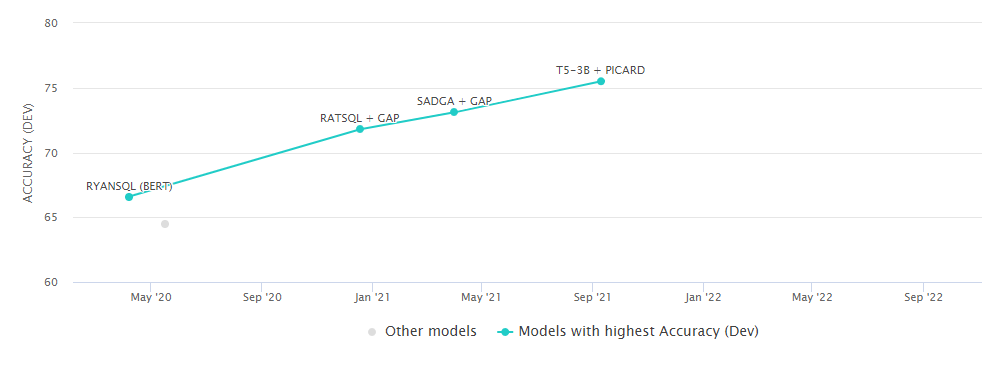
\includegraphics[width=0.9\textwidth]{pics/picard/spider.png}
    \caption{SPIDER Benchmark until 2022}
\end{figure}

T5 Model implemented by Raffel et al. (2020)\cite{raffel_exploring_2020} uses the BERT encoder-decoder architecture proposed by Vaswani et al. (2017) \cite{devlin-etal-2019-bert} and they showed in their studies that it will outperform decoder-only language models. Originally T5 was introduced with five pre-trained models — Small (60 million parameters), Base(220 million parameters), Large(770 million parameters), 3B(3 billion parameters), and 11B(11 billion parameters)\cite{raffel_exploring_2020}. We used the base model in this research due to hardware limitations while fine-tuning for our project.

\begin{figure}[h]
    \centering
    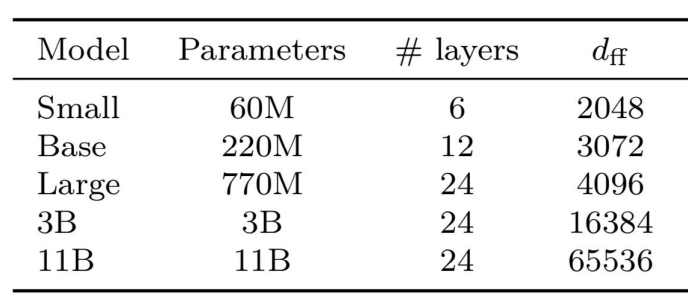
\includegraphics[width=0.5\textwidth]{pics/picard/t5-size.png}
    \caption{T5 models with their Nr. of parameters, layer and feed-forward parameters\cite{raffel_exploring_2020}}
\end{figure}

To pre-train the T5 model, we start with clean text and drop some words to corrupt the text. Each dropped-out span will be replaced with a unique sentinel token, so if multiple words in a row get dropped out, they will be replaced with a single token. The words are dropped out independently uniformly at random so for an inviting get replaced by a single Sentinel token. Then the model is trained to output Sentinel tokens to delineate the dropped-out text corresponding to the text that was dropped out in the input and then each span of dropped-out text.

This method is pretty similar to the span BERT objective. It tried to come up with an objective that was not too different from standard practice.

\begin{figure}[h]
    \centering
    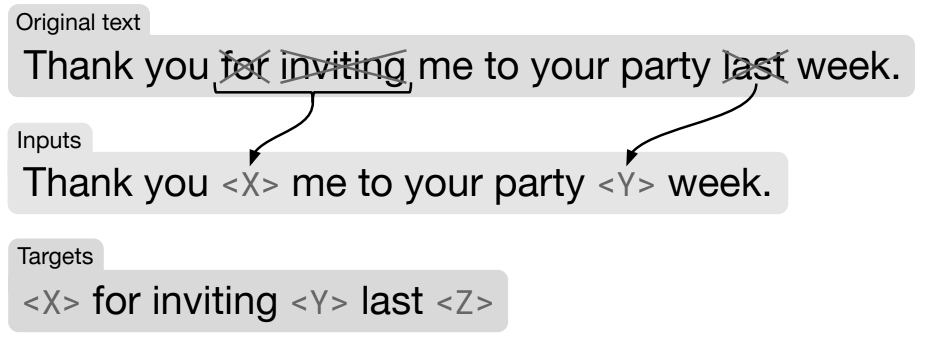
\includegraphics[width=0.6\textwidth]{pics/picard/t5-fine.png}
    \caption{Pre-training by Replace Corrupted Spans \cite{raffel_exploring_2020}}
\end{figure}

Google T5's basic idea is that it models every NLP problem and every text problem as a text-to-text task that takes the text as input and produces text as output.

So fundamentally, it is in a sequence-to-sequence framework, and hence T5 is perfectly suitable for transfer learning machine translation.
T5 can handle various tasks, and it can be fine-tuned for different NLP tasks, such as summarization, COLA (Corpus on linguistic acceptability), classification, multiple text translation, also regression problems like STSB  that predict how similar two sentences are.

\begin{figure}[h]
    \centering
    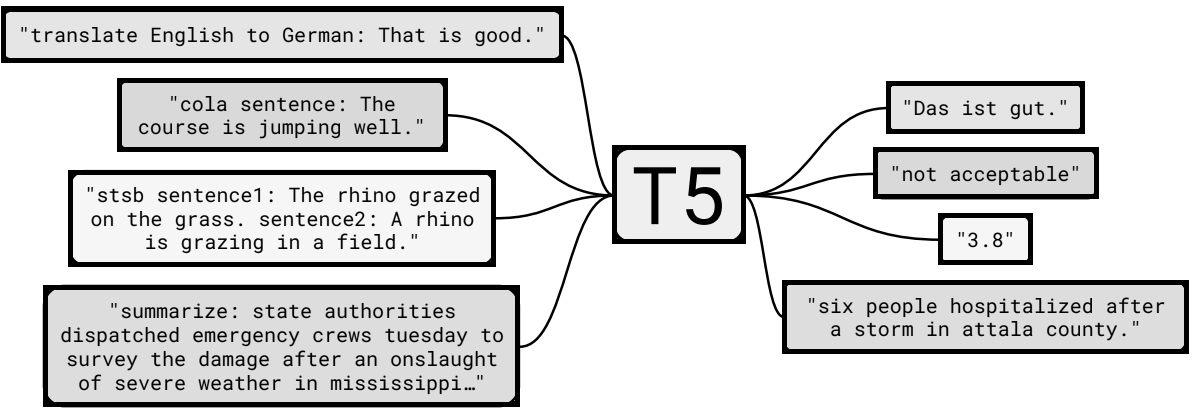
\includegraphics[width=0.9\textwidth]{pics/picard/t5-task.png}
    \caption{Each task uses text as input in the model and generates target text. In this way, the same model, loss function, and hyper-parameters are used across various diverse tasks, including translation. \cite{raffel_exploring_2020}}
\end{figure}

Further, because the same model is used for many tasks, the model understands which tasks to perform by prepending a prefix that will also be text.
Therefore, By the end of fine-tuning, T5 will have "n" different models where "n" is the number of tasks. It starts with the same base pre-trained model, and then it is fine-tuned on task A, and then separately, on task B and task C. In our work, we are essentially adding another task to the T5 to handle SQL translation.

\subsubsection*{C4 (Colossal Clean Crawled Corpus)}

The T5 model is pre-trained on C4 Dataset\cite{raffel_exploring_2020}, so its results are quite realistic.
The C4 is an unlabeled dataset gathered and filtered from Common Crawl Dataset, a non-commercial crawler that saves snapshots of the web every month. And web content is dumped out on the order of 20 terabytes.

The cleaning process included deduplication, discarding incomplete sentences, and removing offensive or noisy content. The filtering led to more reliable results on downstream tasks, and the added size let the model size grow without over-fitting when pre-training. C4 is about 750 gigabytes of clean-ish data and is accessible in Tensorflow Datasets Library.